\chapter{Fundamentação Teórica}
\label{cap:fund}

Este capítulo apresenta os conceitos teóricos fundamentais para a compreensão deste trabalho. A estrutura inicia com a caracterização das imagens hiperespectrais, objeto central deste estudo, seguida pelas técnicas de processamento de imagens e segmentação utilizadas no pré-processamento espacial. Na sequência, são abordados os fundamentos de aprendizado de máquina e aprendizado profundo, com ênfase nas redes neurais convolucionais unidimensionais empregadas na classificação espectral. O capítulo inclui também os conceitos de processamento paralelo em GPUs e encerra com a análise dos trabalhos relacionados que fundamentam a proposta metodológica.

\section{Imagem Hiperespectral}

As imagens hiperespectrais constituem o tipo de dado central deste trabalho, sendo utilizadas como entrada para o processo de classificação. Esta seção apresenta os conceitos fundamentais sobre a estrutura, aquisição e características das HSIs, bem como os desafios associados à sua análise e as técnicas de redução de dimensionalidade empregadas para mitigá-los.

A imagem hiperespectral (HSI) combina espectroscopia e imagem, capturando informações tanto no domínio espacial quanto no espectral \cite{Li2019DeepLF}. Enquanto imagens multiespectrais convencionais capturam poucas bandas em faixas largas do espectro, as HSIs registram centenas de bandas espectrais estreitas e contíguas, tipicamente na faixa de 400 a 2500 nanômetros \cite{Qian2020}. O espectro eletromagnético pode ser organizado de acordo com a energia por fóton, variando de raios gama (maior energia) a ondas de rádio (menor energia) \cite{gonzalez2018digital}. As imagens hiperespectrais capturam informações em múltiplas bandas espectrais estreitas e contíguas, permitindo análise detalhada da composição dos materiais em uma cena. A Figura \ref{fig:landsat_bands} mostra imagens de satélite LANDSAT da área de Washington D.C. em diferentes bandas espectrais temáticas, ilustrando como diferentes bandas do espectro revelam características distintas da superfície terrestre. A HSI tem aplicações em sensoriamento remoto, agricultura de precisão e diagnóstico médico \cite{Lurs12162659}.

\begin{figure}[H]
    \centering
    \captionsetup{justification=centering}
    \caption{Imagens de satélite LANDSAT da área de Washington D.C. em diferentes bandas espectrais temáticas}
    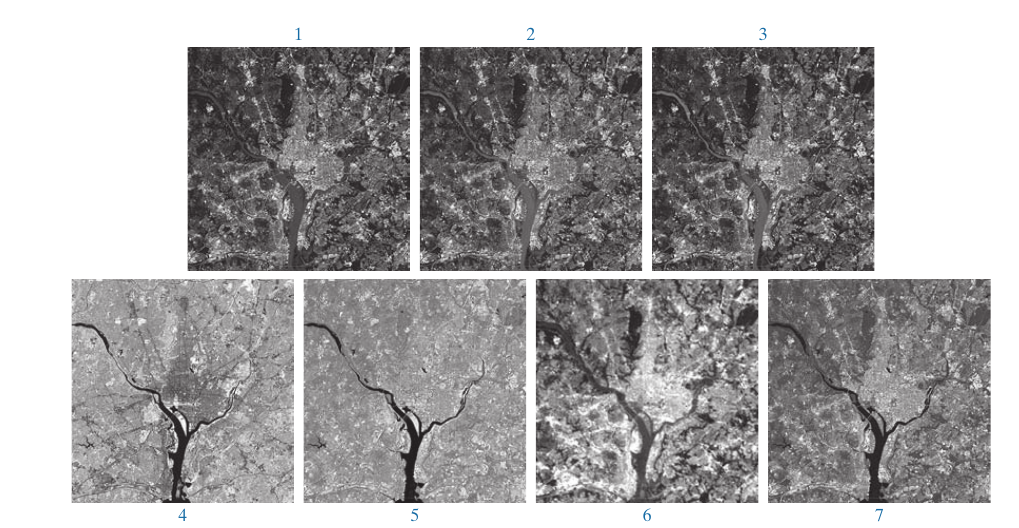
\includegraphics[width=0.95\textwidth]{assets/fundamentacao/landsat_bands.png}
    \captionsetup{justification=raggedright}
    \caption*{Fonte: \citefigure{gonzalez2018digital}}
    \label{fig:landsat_bands}
\end{figure}

A alta dimensionalidade e redundância de dados inerentes às HSIs apresentam desafios computacionais que exigem técnicas de processamento especializadas. Uma HSI possui alta resolução espectral mas baixa resolução espacial \cite{Viel2019}. Essa característica resulta do foco do sensor em capturar um único ponto da cena em centenas de frequências de banda estreita e contíguas. A Figura \ref{fig:hsi_structure} ilustra a estrutura de dados de uma HSI, mostrando como a plataforma de sensor em movimento captura linhas de varredura sucessivas que são empilhadas para formar um hipercubo tridimensional, combinando espectroscopia com imagem para obter informações espectrais e espaciais simultaneamente.

\begin{figure}[H]
    \centering
    \captionsetup{justification=centering}
    \caption{Estrutura de dados de uma imagem hiperespectral: (a) aquisição por sensor em movimento; (b) formação do hipercubo tridimensional; (c) dimensões espaciais e canais espectrais}
    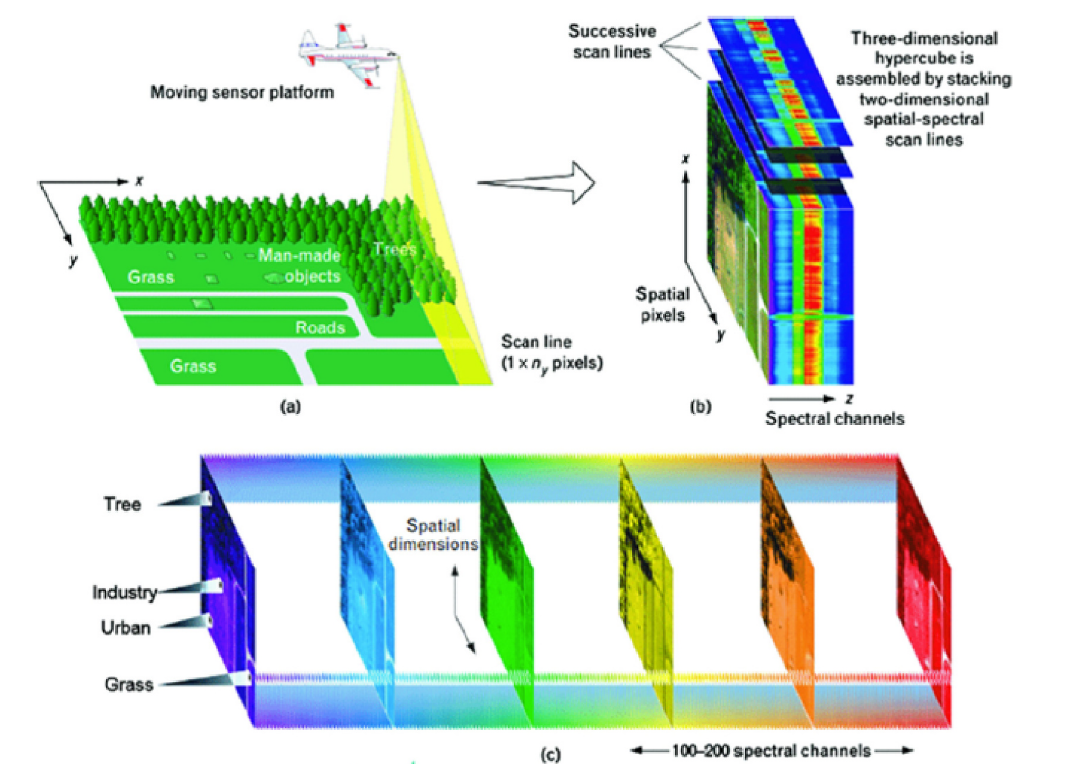
\includegraphics[width=0.95\textwidth]{assets/fundamentacao/hsi_structure.png}
    \captionsetup{justification=raggedright}
    \caption*{Fonte: \citefigure{Qian2020}}
    \label{fig:hsi_structure}
\end{figure}

A análise de dados hiperespectrais enfrenta desafios devido à sua alta dimensionalidade. Os principais desafios são: (1) alta redundância de dados, causada pela forte correlação entre bandas espectrais adjacentes; (2) variabilidade das assinaturas hiperespectrais, que podem mudar devido a condições atmosféricas ou de iluminação; e (3) a "maldição da dimensionalidade" (curse of dimensionality), onde o grande número de bandas espectrais afeta negativamente o desempenho de algoritmos de classificação, exigindo um número exponencialmente maior de amostras de treinamento \cite{Ahmad_2025}. As etapas básicas para análise de HSIs incluem pré-processamento, extração e seleção de características, e classificação ou desmistura (unmixing) espectral.

\subsection{Redução de Dimensionalidade}

Dado o elevado número de bandas espectrais presentes nas HSIs, técnicas de redução de dimensionalidade são necessárias para mitigar os desafios computacionais e estatísticos associados. Esta subseção apresenta a Análise de Componentes Principais (PCA), método amplamente utilizado para projetar os dados em um espaço de menor dimensão preservando a maior parte da variância.

A projeção dos dados por PCA é definida pela equação:

\begin{equation}
z_i^t = w_i^T x^t, \quad i=1,\ldots,k, \quad t=1,\ldots,N
\end{equation}
\addEquacao{Projeção PCA}{6}

\noindent onde $x^t$ são os dados de entrada do pixel $t$, $w_i$ são os autovetores correspondentes aos maiores autovalores, $z_i^t$ são as componentes principais projetadas, $k$ é o número de componentes principais retidas, e $N$ é o número total de pixels. O algoritmo PCA envolve: (1) centralização dos dados subtraindo a média espectral; (2) cálculo da matriz de covariância; (3) decomposição da matriz de covariância em autovetores e autovalores; e (4) projeção dos dados originais nos autovetores correspondentes aos maiores autovalores.

\section{Processamento de Imagens}

O processamento de imagens fornece as técnicas fundamentais para manipulação e análise dos dados visuais, incluindo as operações de pré-processamento e segmentação utilizadas neste trabalho. Esta seção apresenta os conceitos básicos de processamento digital de imagens e seus diferentes níveis de abstração, estabelecendo a base para a compreensão das técnicas de segmentação aplicadas às HSIs.

Uma imagem pode ser definida como uma função bidimensional, $f(x, y)$, onde $x$ e $y$ são coordenadas espaciais, e a amplitude de $f$ em qualquer par de coordenadas $(x, y)$ é chamada de intensidade ou nível de cinza da imagem naquele ponto \cite{gonzalez2018digital}. Quando $x$, $y$ e os valores de intensidade de $f$ são quantidades finitas e discretas, a imagem é chamada de imagem digital. O campo do processamento digital de imagens refere-se ao processamento de imagens digitais por meio de um computador digital.

O processamento de imagens pode ser categorizado em três níveis: baixo nível (pré-processamento, redução de ruído, realce de contraste), nível médio (segmentação, descrição de objetos, classificação) e alto nível (análise de cena e reconhecimento). A Figura \ref{fig:erosion_example} exemplifica uma operação morfológica de erosão, um tipo de processamento de baixo nível comumente utilizado para remover componentes indesejados de imagens binárias.

\begin{figure}[H]
    \centering
    \captionsetup{justification=centering}
    \caption{Exemplo de operação de erosão morfológica aplicada a uma imagem binária usando elementos estruturantes de diferentes tamanhos}
    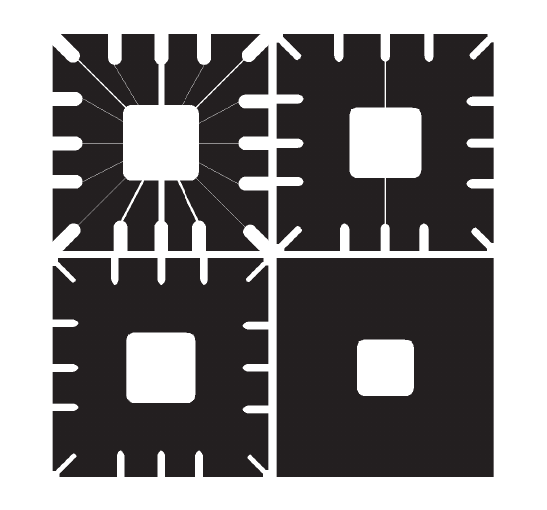
\includegraphics[width=0.75\textwidth]{assets/fundamentacao/erosion_example.png}
    \captionsetup{justification=raggedright}
    \caption*{Fonte: \citefigure{gonzalez2018digital}}
    \label{fig:erosion_example}
\end{figure}

A Figura \ref{fig:segmentation_cells} exemplifica o processamento de nível médio, mostrando a segmentação e identificação de células individuais em imagens microscópicas.

\begin{figure}[H]
    \centering
    \captionsetup{justification=centering}
    \caption{Exemplo de processamento de nível médio: segmentação de células em imagens microscópicas}
    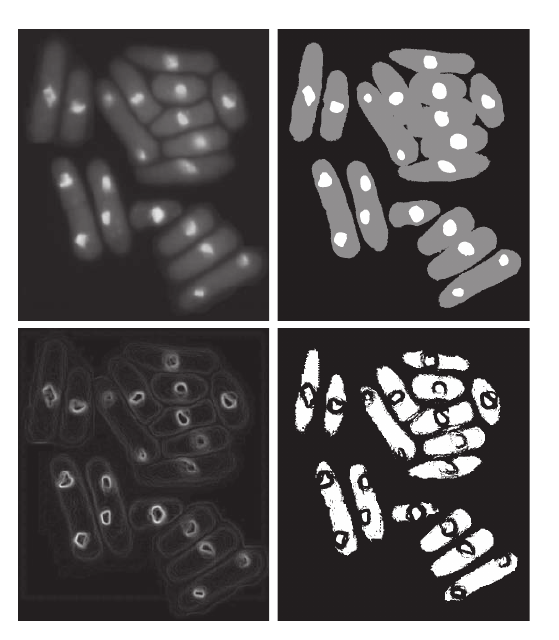
\includegraphics[width=0.65\textwidth]{assets/fundamentacao/segmentation_cells.png}
    \captionsetup{justification=raggedright}
    \caption*{Fonte: \citefigure{gonzalez2018digital}}
    \label{fig:segmentation_cells}
\end{figure}

A Figura \ref{fig:sift_matching} exemplifica o processamento de alto nível, mostrando o reconhecimento e correspondência de características entre imagens usando o algoritmo SIFT.

\begin{figure}[H]
    \centering
    \captionsetup{justification=centering}
    \caption{Exemplo de processamento de alto nível: correspondência de características usando SIFT, mostrando 41 pares encontrados com apenas 3 erros reais}
    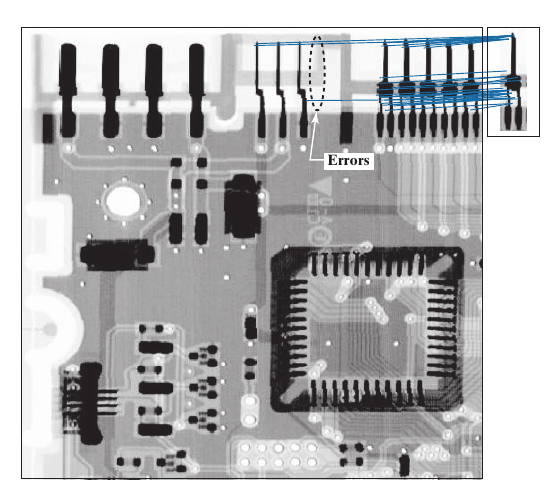
\includegraphics[width=0.55\textwidth]{assets/fundamentacao/sift_matching.png}
    \captionsetup{justification=raggedright}
    \caption*{Fonte: \citefigure{gonzalez2018digital}}
    \label{fig:sift_matching}
\end{figure}

As abordagens tradicionais eram estruturadas em dois módulos: um extrator de características fixo e um classificador treinável. Essa metodologia dependia da engenharia manual de características. O DL permitiu evoluir ao introduzir modelos capazes de aprender automaticamente representações hierárquicas diretamente dos dados brutos.

\subsection{Segmentação de Imagens}

A segmentação constitui uma etapa fundamental no pipeline de classificação proposto neste trabalho, sendo responsável pela extração de informações espaciais que complementam as características espectrais. Esta subseção apresenta os conceitos de segmentação, os algoritmos baseados em superpixels (SEEDS, LSC e Watershed) e as métricas de avaliação utilizadas para quantificar o desempenho da classificação.

A segmentação de imagens é o processo de particionar uma imagem em múltiplos segmentos ou regiões de interesse \cite{FENG2019309}. Sua função é simplificar a representação de uma imagem em algo mais fácil de analisar. No domínio das HSIs, a segmentação utiliza dados espaciais para auxiliar no processo de classificação, o que é útil quando objetos distintos apresentam assinaturas espectrais idênticas mas possuem estruturas geométricas ou texturas diferentes \cite{Souza2023}. A Figura \ref{fig:segmentation_types} ilustra os dois principais tipos de mapa de segmentação gerados pelo algoritmo SEEDS: o mapa de bordas, que identifica os contornos entre superpixels, e o mapa de regiões, que atribui rótulos únicos a cada segmento homogêneo da imagem.

\begin{figure}[H]
    \centering
    \captionsetup{justification=centering}
    \caption{Tipos de mapa de segmentação: bordas (superior) e regiões (inferior) gerados pelo algoritmo SEEDS}
    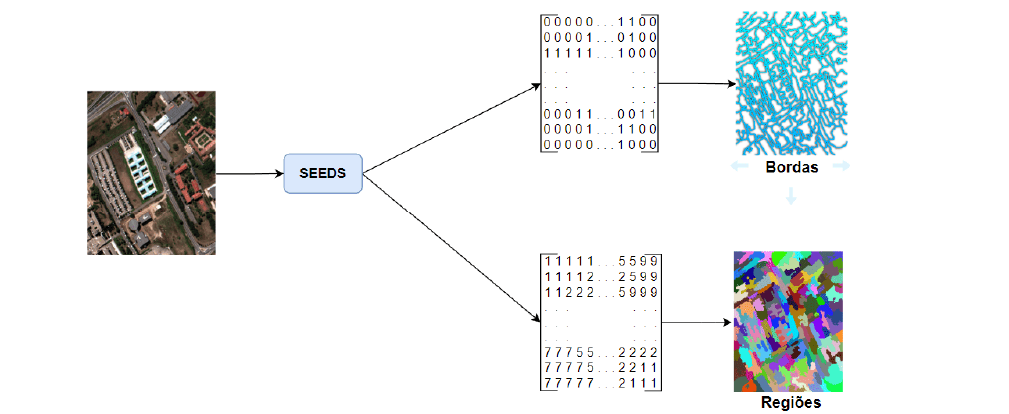
\includegraphics[width=0.85\textwidth]{assets/fundamentacao/segmentation_types.png}
    \captionsetup{justification=raggedright}
    \caption*{Fonte: \citefigure{Souza2023}}
    \label{fig:segmentation_types}
\end{figure}

Um método de segmentação morfológica utiliza os resíduos de transformadas de abertura e fechamento morfológicas baseadas em uma métrica geodésica \cite{Pesaresi905239}. Essa abordagem introduz o conceito de "nivelamento" (leveling). A reconstrução em tons de cinza de uma imagem g a partir de um marcador f é obtida pelo uso iterativo de dilatações geodésicas elementares até a idempotência:

\begin{equation}
R_g^\delta(f) = \delta_g^{(i)}(f)
\end{equation}
\addEquacao{Reconstrução Geodésica Morfológica}{7}

\noindent onde $R_g^\delta(f)$ é a reconstrução geodésica da imagem $f$ sob a imagem de referência $g$, e $\delta_g^{(i)}(f)$ representa a dilatação geodésica elementar aplicada iterativamente até atingir idempotência (estabilidade). A característica morfológica multiescala de um ponto na imagem é definida pelo tamanho do elemento estruturante que possui o maior valor associado na derivada do perfil morfológico. O vetor da derivada do perfil morfológico (DMP) é:

\begin{equation}
\Delta(x) = (\Delta_0(x), ..., \Delta_\lambda(x), ..., \Delta_N(x))
\end{equation}
\addEquacao{Vetor de Derivada do Perfil Morfológico (DMP)}{8}

\noindent onde $\Delta(x)$ é o vetor de derivadas do perfil morfológico no ponto $x$, $\Delta_\lambda(x)$ representa a derivada para o elemento estruturante de tamanho $\lambda$, e $N$ é o número total de escalas. O algoritmo SEEDS (Superpixels Extracted via Energy-Driven Sampling) utiliza uma função de energia para particionar a imagem:

\begin{equation}
E(s) = H(s) + \gamma G(s)
\end{equation}
\addEquacao{Função de Energia do Algoritmo SEEDS}{9}

\noindent onde $E(s)$ é a função de energia total da segmentação $s$, $H(s)$ é o termo de histograma que mede a homogeneidade de cor dentro dos superpixels, $G(s)$ é o termo de penalização de contorno que incentiva bordas suaves, e $\gamma$ é o parâmetro que controla o equilíbrio entre cor e contornos.

\subsection{Métricas de Avaliação}

A avaliação quantitativa do desempenho de classificação requer métricas padronizadas que permitam comparação objetiva entre diferentes abordagens. Esta subseção apresenta as principais métricas utilizadas na classificação de HSIs, incluindo medidas de acurácia e o coeficiente Kappa para avaliação da concordância.

\textbf{Acurácia Geral (Overall Accuracy - OA):}

\begin{equation}
OA = \frac{vp + vn}{vp + vn + fp + fn}
\end{equation}
\addEquacao{Acurácia Geral (OA)}{10}

\noindent onde $vp$ são os verdadeiros positivos, $vn$ são os verdadeiros negativos, $fp$ são os falsos positivos, e $fn$ são os falsos negativos. Esta métrica representa a proporção total de pixels corretamente classificados.

\textbf{Acurácia Média (Average Accuracy - AA):}

\begin{equation}
AA = \frac{1}{n_{classes}} \sum_{i=1}^{n_{classes}} \text{Acurácia}_{\text{Classe}_i}
\end{equation}
\addEquacao{Acurácia Média (AA)}{11}

\noindent onde $n_{classes}$ é o número total de classes e $\text{Acurácia}_{\text{Classe}_i}$ é a acurácia de classificação para a classe $i$.

\textbf{Coeficiente Kappa ($\kappa$):}

\begin{equation}
\kappa = \frac{p_o - p_e}{1 - p_e}
\end{equation}
\addEquacao{Coeficiente Kappa}{12}

\noindent onde $p_o$ é a acurácia observada (concordância real) e $p_e$ é a acurácia esperada (concordância por acaso). O coeficiente Kappa avalia o grau de concordância entre a classificação e o Ground Truth (GT), ajustando para concordâncias que ocorreriam por acaso.

\section{Aprendizado de Máquina}

O aprendizado de máquina fornece os fundamentos teóricos para os modelos de classificação empregados neste trabalho. Esta seção apresenta os conceitos fundamentais de ML, desde a definição formal de aprendizado até os paradigmas de aprendizagem, estabelecendo a base para a compreensão das redes neurais convolucionais utilizadas na classificação espectral de HSIs.

O Aprendizado de Máquina, do inglês \textit{Machine Learning} (ML), é um campo de estudo que confere aos computadores a capacidade de aprender sem serem explicitamente programados \cite{SomeStudiesinMachineLearningUsingtheGameofCheckers}. Este campo abrange desde algoritmos clássicos até arquiteturas de aprendizado profundo, como CNNs e TFs \cite{DeeplearningLC}. Um programa de computador aprende a partir de uma experiência ($E$) com respeito a uma classe de tarefas ($T$) e uma medida de desempenho ($P$), se o seu desempenho nas tarefas em $T$, medido por $P$, melhora com a experiência $E$ \cite{MachineLearning}. A Figura \ref{fig:checkers_tree} ilustra um exemplo clássico de aprendizado de máquina aplicado ao jogo de damas, onde o sistema avalia possíveis movimentos através de uma árvore de decisão, escolhendo o ramo com maior pontuação.

\begin{figure}[H]
    \centering
    \captionsetup{justification=centering}
    \caption{Diagrama simplificado mostrando como as avaliações são respaldadas através da árvore de movimentos possíveis para chegar ao melhor próximo movimento}
    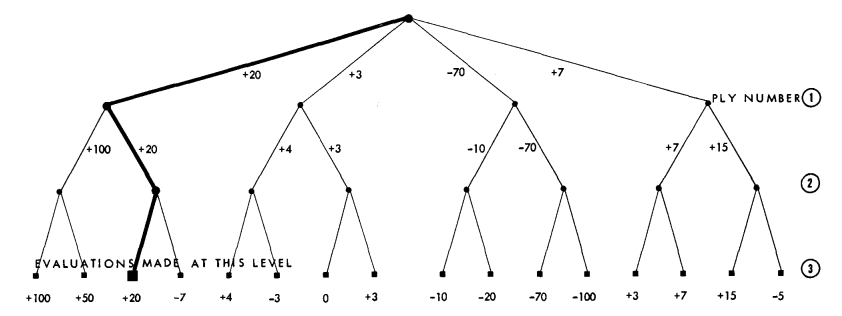
\includegraphics[width=0.75\textwidth]{assets/fundamentacao/checkers_tree.png}
    \captionsetup{justification=raggedright}
    \caption*{Fonte: \citefigure{SomeStudiesinMachineLearningUsingtheGameofCheckers}}
    \label{fig:checkers_tree}
\end{figure}

\subsection{Desafios Centrais: Generalização e Sobreajuste}

O desenvolvimento de modelos de aprendizado de máquina eficazes requer atenção aos problemas de generalização e sobreajuste, que afetam diretamente a capacidade do modelo de performar adequadamente em dados não vistos durante o treinamento. Esta subseção aborda esses desafios e as estratégias de regularização empregadas para mitigá-los.

O desafio principal é garantir que o desempenho de um modelo ($P$) melhore não apenas nos dados de treinamento ($E$), mas também em dados novos. Quando isso não ocorre, há sobreajuste, do inglês \textit{overfitting} (OF), onde o modelo se ajusta excessivamente aos dados de treinamento, capturando ruídos em vez do padrão subjacente \cite{Overfittingproblem:anewperspectivefromthegeometricalinterpretationofMLP}. O OF resulta em bom desempenho no treinamento mas performance ruim em novas entradas. A Figura \ref{fig:gradient_descent} ilustra um comportamento durante o treinamento: a norma do gradiente aumenta ao longo do tempo e épocas com o erro de classificação no conjunto de validação diminuindo para um nível baixo. Estratégias de regularização são empregadas para restringir a complexidade do modelo e evitar o OF \cite{Dropout:asimplewaytopreventneuralnetworksfromoverfitting}.

\begin{figure}[H]
    \centering
    \captionsetup{justification=centering}
    \caption{Comportamento da descida de gradiente durante o treinamento de uma rede convolucional: (Esquerda) distribuição das normas do gradiente ao longo do tempo; (Direita) taxa de erro de classificação no conjunto de validação}
    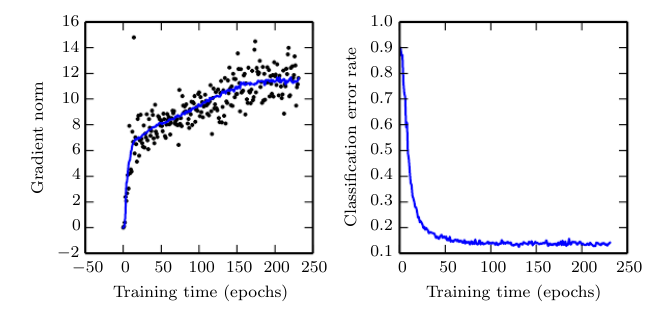
\includegraphics[width=0.85\textwidth]{assets/fundamentacao/gradient_descent_behavior.png}
    \captionsetup{justification=raggedright}
    \caption*{Fonte: \citefigure{DeepLearningIG}}
    \label{fig:gradient_descent}
\end{figure}

\subsection{Paradigmas de Aprendizagem}

A escolha do paradigma de aprendizagem adequado depende da natureza dos dados disponíveis e do problema a ser resolvido. Esta subseção apresenta os três principais paradigmas — supervisionado, não supervisionado e semissupervisionado — contextualizando a abordagem supervisionada utilizada neste trabalho para classificação de HSIs.

A natureza dos dados e do problema determina qual paradigma de aprendizado usar \cite{WhatIsMachineLearning}. A Figura \ref{fig:learning_paradigms} ilustra os três principais paradigmas de aprendizagem e como eles se relacionam com os diferentes tipos de dados de treinamento.

\begin{figure}[H]
    \centering
    \captionsetup{justification=centering}
    \caption{Paradigmas de aprendizagem e sua relação com os tipos de dados de treinamento}
    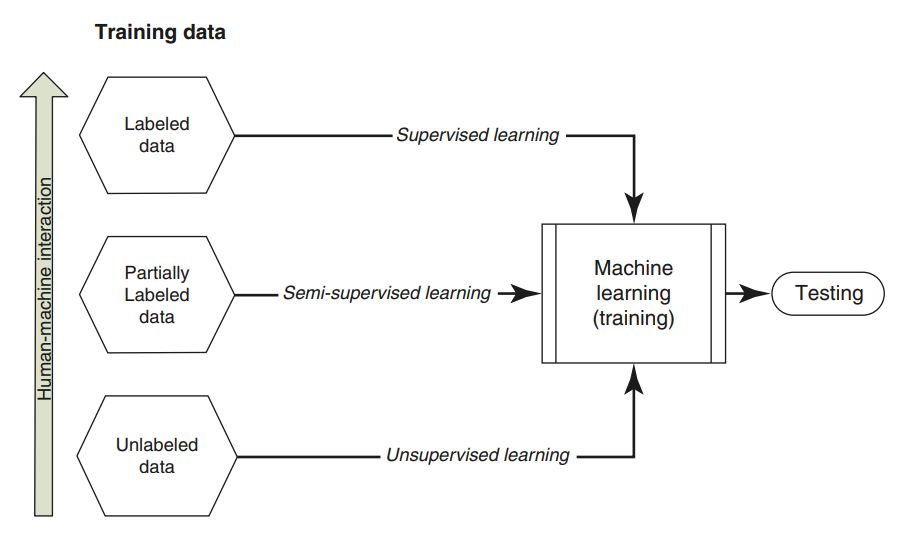
\includegraphics[width=0.75\textwidth]{assets/fundamentacao/learning_paradigms.png}
    \captionsetup{justification=raggedright}
    \caption*{Fonte: \citefigure{WhatIsMachineLearning}}
    \label{fig:learning_paradigms}
\end{figure}

\begin{itemize}
    \item \textbf{Aprendizado Supervisionado}: Estima um mapeamento a partir de amostras de entrada e saída, onde as saídas são rótulos ou valores conhecidos. As tarefas mais comuns são classificação e regressão.

    \item \textbf{Aprendizado não supervisionado}: O sistema recebe apenas amostras de entrada, sem rótulos.

    \item \textbf{Aprendizado Semissupervisionado}: Do inglês \textit{Semi-supervised learning} (SSL), se situa entre os paradigmas supervisionado e não supervisionado, usando dados onde apenas parte das amostras é rotulada.
\end{itemize}

\subsection{Aprendizado Profundo}

O aprendizado profundo representa a evolução das técnicas de ML que possibilita a extração automática de características hierárquicas dos dados. Esta subseção apresenta os fundamentos do DL, incluindo as funções de ativação, o algoritmo de retropropagação e as arquiteturas de redes neurais convolucionais, com ênfase nas CNNs 1D empregadas na classificação espectral de HSIs.

O Aprendizado Profundo, do inglês \textit{Deep Learning} (DL), permite que modelos compostos por múltiplas camadas de processamento aprendam representações de dados com múltiplos níveis de abstração \cite{Asurveyonstate-of-the-artdeeplearningapplicationsandchallenges}. O DL é um método de aprendizado de representação com múltiplos níveis, obtido pela composição de módulos simples e não lineares \cite{DeeplearningLC}. Cada camada transforma a representação da camada anterior em um nível de abstração superior. A Figura \ref{fig:cnn_architecture} ilustra a arquitetura de uma rede neural convolucional, mostrando as operações de convolução com função de ativação ReLU e as camadas de max pooling que reduzem progressivamente a dimensionalidade espacial. As funções de ativação, como a Unidade Linear Retificada (ReLU), introduzem não-linearidades. A função ReLU é definida como:

\begin{equation}
f(z) = \max(z, 0) = \begin{cases} 
z, & \text{se } z > 0 \\
0, & \text{caso contrário}
\end{cases}
\end{equation}
\addEquacao{Função de Ativação ReLU}{1}

\noindent onde $z$ é a entrada da função de ativação. A ReLU acelera o processo de aprendizado em comparação com a sigmoide ou tangente hiperbólica devido à sua simplicidade computacional. O treinamento dessas redes usa o algoritmo de retropropagação, do inglês \textit{backpropagation}, que calcula o gradiente da função de perda em relação a cada peso na rede, permitindo o ajuste dos parâmetros por descida de gradiente \cite{Gradient-basedlearningappliedtodocumentrecognition}. A Figura \ref{fig:backpropagation} ilustra como uma rede neural multicamadas pode distorcer o espaço de entrada para tornar as classes de dados linearmente separáveis, e demonstra o processo de backpropagation através da regra da cadeia, mostrando tanto o forward pass (propagação para frente) quanto o backward pass (retropropagação dos gradientes).

\begin{figure}[H]
    \centering
    \captionsetup{justification=centering}
    \caption{Redes neurais multicamadas e backpropagation: (a) transformação do espaço de entrada; (b) regra da cadeia; (c) equações do forward pass; (d) equações do backward pass}
    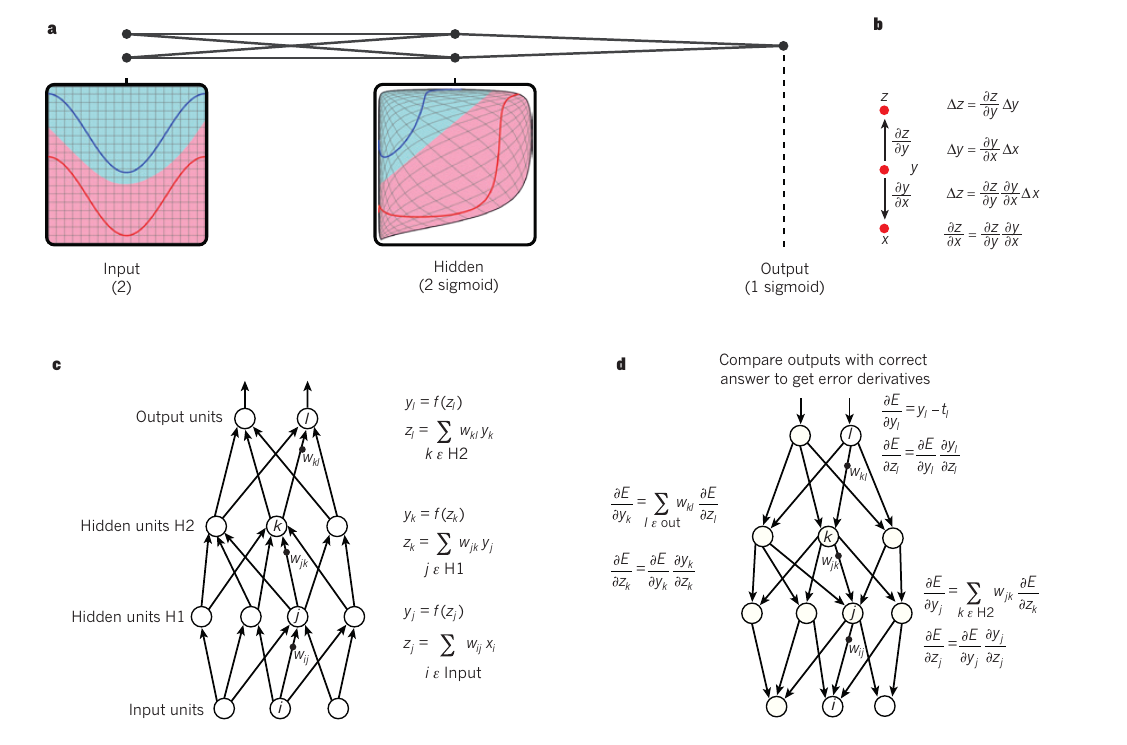
\includegraphics[width=0.95\textwidth]{assets/fundamentacao/backpropagation.png}
    \captionsetup{justification=raggedright}
    \caption*{Fonte: \citefigure{DeeplearningLC}}
    \label{fig:backpropagation}
\end{figure}

\begin{figure}[H]
    \centering
    \captionsetup{justification=centering}
    \caption{Arquitetura de uma rede neural convolucional mostrando camadas de convolução com ReLU e max pooling}
    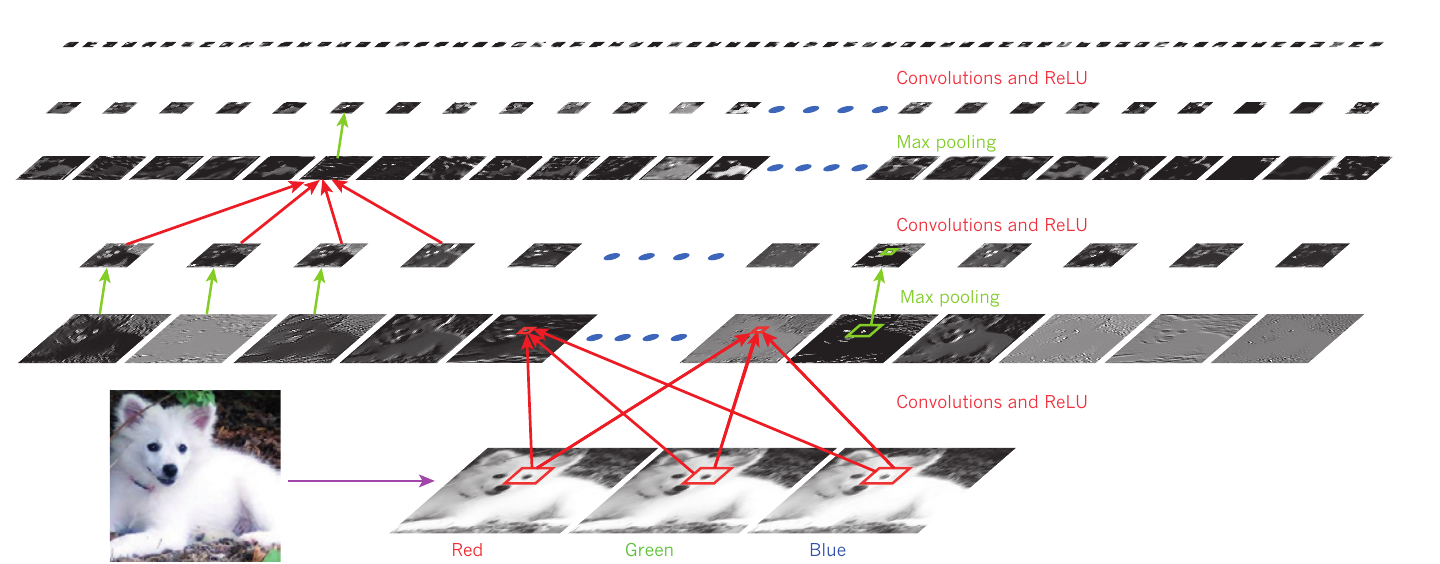
\includegraphics[width=0.9\textwidth]{assets/fundamentacao/cnn_architecture.png}
    \captionsetup{justification=raggedright}
    \caption*{Fonte: \citefigure{DeeplearningLC}}
    \label{fig:cnn_architecture}
\end{figure}

O treinamento de redes neurais profundas depende de algoritmos de otimização estocástica para ajustar os parâmetros do modelo \cite{kingma2017adammethodstochasticoptimization}. O gradiente é definido como:

\begin{equation}
\nabla_{\theta} L = \frac{\partial L}{\partial \theta}
\end{equation}
\addEquacao{Gradiente da Função de Perda}{2}

\noindent onde $\nabla_{\theta}$ é o operador gradiente, $L$ é a função de perda, e $\theta$ são os parâmetros do modelo. A função de perda Erro Quadrático Médio (MSE) é definida como:

\begin{equation}
E(g_X) = \frac{1}{N} \sum_{t=1}^{N} \left[r^t - g(x^t)\right]^2
\end{equation}
\addEquacao{Erro Quadrático Médio (MSE)}{3}

\noindent onde $N$ é o número de amostras, $r^t$ é o valor real (ground truth) da amostra $t$, e $g(x^t)$ é a predição do modelo para a entrada $x^t$.

\subsubsection{Redes Neurais Convolucionais}

As redes neurais convolucionais constituem a arquitetura base para o modelo de classificação espectral deste trabalho. Esta subseção detalha os princípios de funcionamento das CNNs, incluindo a operação de convolução, conexões locais, pesos compartilhados e camadas de pooling, culminando na apresentação da arquitetura CNN 1D específica para classificação de HSIs.

As CNNs são um tipo especializado de rede neural projetada para processar dados com topologia de grade \cite{DeepLearningIG}. Sua arquitetura se baseia em quatro ideias: conexões locais, pesos compartilhados, agrupamento (pooling) e uso de múltiplas camadas. A operação de convolução em uma dimensão (1D) é definida como:

\begin{equation}
s(t) = (x \ast w)(t) = \sum_{a=-\infty}^{\infty} x(a) \cdot w(t-a)
\end{equation}
\addEquacao{Operação de Convolução 1D}{4}

\noindent onde $x$ é o sinal de entrada, $w$ o kernel (filtro) da convolução, e $s(t)$ o resultado da operação no instante $t$. A Figura \ref{fig:convolution_operation} ilustra visualmente como o kernel é aplicado sobre a matriz de entrada durante a operação de convolução. Esta operação é usada na CNN 1D para classificação espectral de imagens hiperespectrais.

\begin{figure}[H]
    \centering
    \captionsetup{justification=centering}
    \caption{Operação de convolução mostrando a aplicação do kernel sobre a matriz de entrada}
    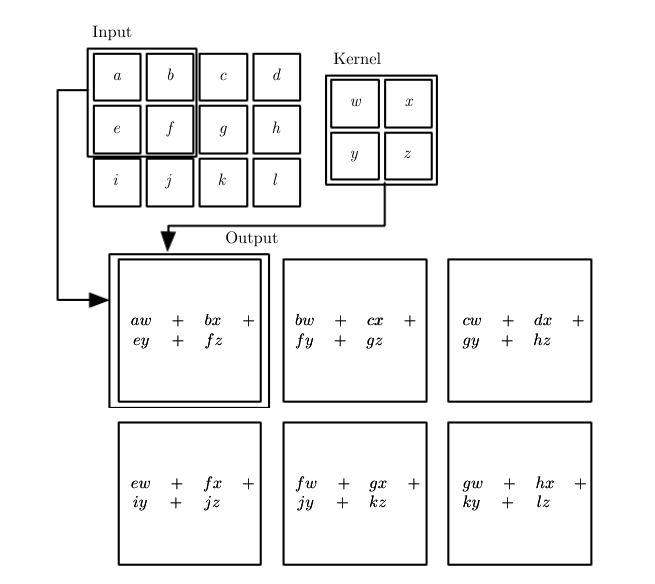
\includegraphics[width=0.75\textwidth]{assets/fundamentacao/convolution_operation.png}
    \captionsetup{justification=raggedright}
    \caption*{Fonte: \citefigure{DeeplearningLC}}
    \label{fig:convolution_operation}
\end{figure}

\noindent Em vez de conectar cada neurônio de uma camada a todos os neurônios da camada anterior, os neurônios em uma camada convolucional são conectados apenas a uma região local (conexões locais) \cite{DeeplearningLC}. A entrada líquida (net input) em um neurônio convolucional é:

\begin{equation}
z_{x,y}^{\ell} = b^{\ell} + \sum_{l,k} w_{l,k}^{\ell} \cdot a_{x-l,y-k}^{\ell-1}
\end{equation}
\addEquacao{Entrada Líquida em Camada Convolucional}{5}

\noindent onde $z_{x,y}^{\ell}$ é a entrada na posição $(x,y)$ da camada $\ell$, $b^{\ell}$ é o viés (bias), $w_{l,k}^{\ell}$ são os pesos do kernel, e $a_{x-l,y-k}^{\ell-1}$ são as ativações da camada anterior. Todas as unidades em um mesmo mapa de características compartilham o mesmo conjunto de pesos, o que reduz o número de parâmetros. Essa abordagem assume que um detector de características útil em uma parte da imagem será útil em outra parte. A camada de pooling reduz a dimensionalidade espacial dos mapas de características, tornando a representação mais compacta e robusta a pequenas translações. Uma CNN típica consiste em estágios de camadas convolucionais seguidas por camadas de pooling, culminando em camadas totalmente conectadas para classificação.

Uma característica fundamental das operações de convolução é a \textbf{independência de dados entre elementos de saída}. Cada elemento do mapa de características de saída pode ser calculado de forma completamente independente dos demais elementos da mesma camada, dependendo apenas de uma região local da entrada e dos pesos do kernel compartilhado. Esta propriedade é crucial para a paralelização eficiente em GPUs, conforme discutido na Seção \ref{sec:paralelismo}.

A evolução das arquiteturas de CNNs é marcada por aumento progressivo em profundidade. Redes pioneiras como a LeNet-5 demonstraram a eficácia da combinação de camadas convolucionais e de pooling para reconhecimento de caracteres \cite{Gradient-basedlearningappliedtodocumentrecognition}. A VGG mostrou que redes profundas podiam ser construídas usando filtros pequenos (3x3) \cite{VeryDeepConvolutionalNetworksforLarge-ScaleImageRecognition}. A GoogLeNet introduziu os módulos "Inception", que executam convoluções de diferentes tamanhos em paralelo \cite{szegedy2014goingdeeperconvolutions}.

\subsubsection{Aplicações de CNNs}

As CNNs possuem ampla aplicabilidade em diferentes domínios de visão computacional. Esta subseção apresenta as principais aplicações, com destaque para a análise de imagens hiperespectrais, que constitui o foco deste trabalho.

As CNNs são usadas em várias aplicações:

\begin{itemize}
    \item \textbf{Classificação de Imagens}: Atribui um único rótulo a uma imagem inteira \cite{NIPS2012_c399862d}.

    \item \textbf{Segmentação Semântica}: Classifica cada pixel de uma imagem em uma categoria específica \cite{Farabet6338939}. É usada em sensoriamento remoto para mapeamento de cobertura do solo.

    \item \textbf{Detecção de Objetos}: Localiza múltiplos objetos em uma imagem por meio de caixas delimitadoras (bounding boxes) e classifica cada um \cite{sermanet2014overfeatintegratedrecognitionlocalization}.

    \item \textbf{Análise de Imagens Hiperespectrais}: Em imagens hiperespectrais, que contêm centenas de bandas espectrais, as CNNs extraem características espectrais e espaciais simultaneamente \cite{Li2019DeepLF}. A Figura \ref{fig:cnn1d_hsi} ilustra uma arquitetura CNN 1D específica para classificação de imagens hiperespectrais, mostrando o fluxo desde o pré-processamento PCA até as camadas convolucionais 1D e densas que produzem a classificação final.
\end{itemize}

\begin{figure}[H]
    \centering
    \captionsetup{justification=centering}
    \caption{Arquitetura CNN 1D para classificação de imagens hiperespectrais: pré-processamento PCA seguido de 4 camadas convolucionais 1D e camadas densas para classificação}
    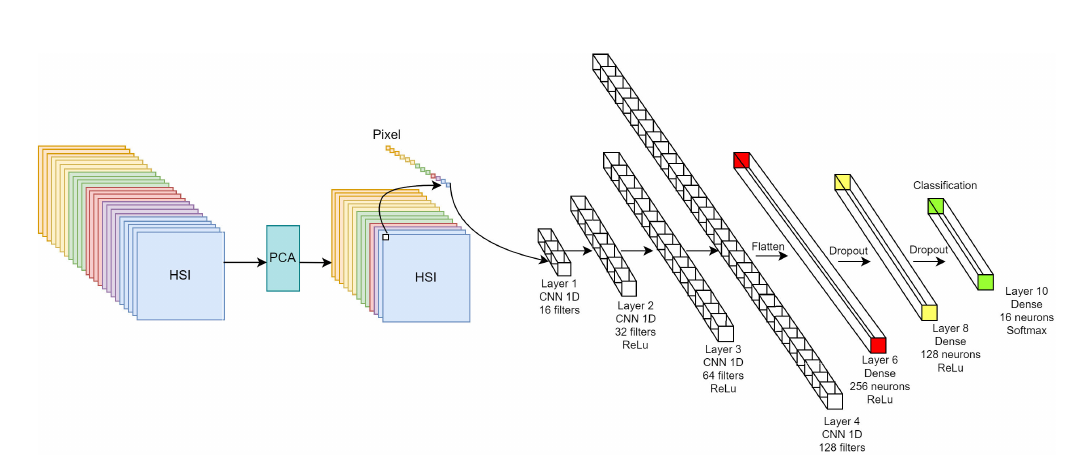
\includegraphics[width=0.95\textwidth]{assets/fundamentacao/cnn1d_hsi_architecture.png}
    \captionsetup{justification=raggedright}
    \caption*{Fonte: \citefigure{Viel10064297}}
    \label{fig:cnn1d_hsi}
\end{figure}

\section{Processamento Paralelo em GPUs}
\label{sec:paralelismo}

O processamento paralelo é uma técnica computacional fundamental para acelerar aplicações de aprendizado profundo. Esta seção apresenta os conceitos de arquitetura de GPUs, a plataforma CUDA e as estratégias de paralelização aplicáveis a CNNs, fundamentando a proposta de paralelização do fluxo de classificação de HSIs.

\subsection{Arquitetura de GPUs e CUDA Cores}

As Unidades de Processamento Gráfico (GPUs) evoluíram de aceleradores gráficos especializados para processadores massivamente paralelos de propósito geral \cite{CUDA_Programming}. Enquanto CPUs modernas possuem tipicamente dezenas de núcleos otimizados para execução sequencial com baixa latência, GPUs NVIDIA contêm milhares de núcleos de processamento denominados \textbf{CUDA cores}, organizados em unidades chamadas Streaming Multiprocessors (SMs). Por exemplo, uma GPU NVIDIA RTX 3080 possui 8704 CUDA cores distribuídos em 68 SMs, enquanto uma GPU A100 para computação científica possui 6912 CUDA cores em 108 SMs.

Cada CUDA core é capaz de executar operações aritméticas de ponto flutuante (soma, multiplicação, operações fusionadas FMA) em um único ciclo de clock. Os CUDA cores dentro de um SM executam instruções seguindo o modelo SIMT (Single Instruction, Multiple Threads), onde grupos de 32 threads chamados \textit{warps} executam a mesma instrução simultaneamente sobre dados diferentes. Esta arquitetura é particularmente eficiente para operações que apresentam paralelismo de dados, onde a mesma operação deve ser aplicada a grandes conjuntos de elementos independentes.

A plataforma CUDA (Compute Unified Device Architecture), desenvolvida pela NVIDIA, fornece um modelo de programação que permite aos desenvolvedores explorar o paralelismo das GPUs para aplicações de computação geral \cite{CUDA_Programming}. O modelo de execução CUDA organiza os threads em uma hierarquia de três níveis: threads individuais são agrupados em blocos (blocks), e blocos são organizados em grades (grids). Esta organização permite escalabilidade automática entre GPUs com diferentes números de SMs, pois o hardware distribui automaticamente os blocos entre os SMs disponíveis.

A memória da GPU também é organizada hierarquicamente para otimizar o desempenho:
\begin{itemize}
    \item \textbf{Memória Global}: Memória principal da GPU (HBM2 ou GDDR6), com alta capacidade (até 80 GB em GPUs datacenter) mas latência elevada (400-600 ciclos).
    \item \textbf{Memória Compartilhada}: Memória on-chip de baixa latência (20-30 ciclos) acessível por todos os threads de um mesmo bloco, tipicamente 48-164 KB por SM.
    \item \textbf{Registradores}: Memória privada de cada thread com latência de 1 ciclo, tipicamente 65536 registradores de 32 bits por SM.
    \item \textbf{Caches L1/L2}: Caches automáticos que reduzem a latência de acesso à memória global.
\end{itemize}

A otimização do padrão de acesso à memória é crítica para o desempenho de aplicações CUDA. Acessos coalescidos, onde threads consecutivos acessam endereços consecutivos de memória, maximizam a largura de banda efetiva \cite{Jorda_cuDNN}.

\subsection{Paralelização de Operações de Convolução}

A operação de convolução em CNNs apresenta características intrínsecas que a tornam altamente paralelizável \cite{cuConv}. Para uma camada convolucional com entrada $X$ de dimensões $(N, C_{in}, H, W)$ (batch, canais de entrada, altura, largura), filtros $K$ de dimensões $(C_{out}, C_{in}, k_h, k_w)$, e saída $Y$ de dimensões $(N, C_{out}, H_{out}, W_{out})$, cada elemento de saída é calculado como:

\begin{equation}
Y[n, c_{out}, i, j] = \sum_{c_{in}=0}^{C_{in}-1} \sum_{m=0}^{k_h-1} \sum_{n=0}^{k_w-1} X[n, c_{in}, i+m, j+n] \cdot K[c_{out}, c_{in}, m, n] + b[c_{out}]
\end{equation}

A propriedade fundamental é que o cálculo de cada elemento $Y[n, c_{out}, i, j]$ é \textbf{completamente independente} do cálculo de qualquer outro elemento da saída. Não existe dependência de dados entre os elementos de saída, significando que todos os $N \times C_{out} \times H_{out} \times W_{out}$ elementos podem ser calculados simultaneamente se houver recursos computacionais suficientes. Em uma CNN 1D para classificação espectral, esta propriedade se mantém: cada posição temporal do mapa de características de saída pode ser calculada em paralelo.

Na prática, frameworks de deep learning como TensorFlow e PyTorch utilizam a biblioteca cuDNN da NVIDIA para implementar operações de convolução otimizadas em GPU \cite{Jorda_cuDNN}. A cuDNN implementa múltiplos algoritmos de convolução:

\begin{itemize}
    \item \textbf{Convolução Direta (IMPLICIT\_GEMM)}: Transforma a convolução em multiplicação de matrizes utilizando a operação im2col, aproveitando bibliotecas BLAS otimizadas.
    \item \textbf{Convolução baseada em FFT}: Utiliza a transformada rápida de Fourier para converter convoluções em multiplicações elemento a elemento no domínio da frequência.
    \item \textbf{Convolução Winograd}: Reduz o número de multiplicações necessárias através de transformações algébricas, eficiente para kernels pequenos (3x3).
\end{itemize}

O cuDNN seleciona automaticamente o algoritmo mais eficiente para cada configuração de parâmetros através de heurísticas ou benchmarking em tempo de execução.

\subsection{Estratégias de Paralelização para o Fluxo de Classificação}

No contexto deste trabalho, diferentes níveis de paralelização podem ser explorados para acelerar o fluxo de classificação de HSIs \cite{Aach2025, Nandan10910577}:

\textbf{Paralelismo de Dados}: Múltiplas réplicas do modelo processam diferentes subconjuntos dos dados de entrada simultaneamente. Os gradientes são agregados para atualização dos pesos. Esta estratégia é implementada pela MirroredStrategy do TensorFlow e DataParallel do PyTorch, sendo particularmente útil quando o dataset é grande e múltiplas GPUs estão disponíveis \cite{Nandan10910577}.

\textbf{Paralelismo Intra-Camada}: Dentro de uma única camada convolucional, as operações sobre diferentes elementos de saída podem ser executadas em paralelo nos CUDA cores. Esta é a forma mais fundamental de paralelismo em CNNs e é automaticamente explorada pelas implementações em GPU.

\textbf{Paralelismo Inter-Etapas}: No contexto específico deste trabalho, as etapas de segmentação espacial e extração de características espectrais pela CNN são processos independentes que podem ser executados concorrentemente. Após o pré-processamento PCA:
\begin{itemize}
    \item A segmentação espacial opera sobre as primeiras componentes principais para gerar o mapa de superpixels. Esta operação pode ser executada em CPU utilizando múltiplas threads através da biblioteca \texttt{multiprocessing} do Python.
    \item A CNN 1D processa os vetores espectrais de cada pixel para extrair características discriminativas. Esta operação é executada em GPU, aproveitando os CUDA cores para paralelização massiva das convoluções.
    \item As duas operações são independentes e não compartilham dados intermediários, permitindo execução simultânea.
    \item A sincronização ocorre apenas no ponto de fusão, onde os resultados de ambas as operações são necessários para a concatenação de características.
\end{itemize}

A implementação de paralelismo em Python pode utilizar diferentes abordagens:
\begin{itemize}
    \item \textbf{multiprocessing}: Cria processos separados com espaços de memória independentes, contornando o Global Interpreter Lock (GIL) do Python. Adequado para operações CPU-bound como algoritmos de segmentação.
    \item \textbf{threading}: Cria threads dentro do mesmo processo. Limitado pelo GIL para código Python puro, mas eficiente para operações que liberam o GIL (como chamadas a bibliotecas C/CUDA).
    \item \textbf{concurrent.futures}: Interface de alto nível que abstrai a criação e gerenciamento de processos ou threads.
\end{itemize}

O speedup teórico máximo da paralelização inter-etapas é determinado pela lei de Amdahl. Se $T_{seg}$ é o tempo de segmentação e $T_{cnn}$ é o tempo da CNN no fluxo sequencial, o tempo do fluxo paralelo será aproximadamente $\max(T_{seg}, T_{cnn}) + T_{overhead}$, onde $T_{overhead}$ representa a sobrecarga de criação de threads e sincronização.

\section{Trabalhos Relacionados}
\label{sec:trabRel}

A análise de trabalhos relacionados permite identificar o estado da arte e as lacunas existentes na literatura que justificam a proposta deste trabalho. Esta seção apresenta o protocolo de busca utilizado, seguido pela análise detalhada de três trabalhos selecionados que abordam temas de otimização relevantes para a classificação de HSIs, e finaliza com uma análise comparativa que posiciona a contribuição deste estudo.

\subsection{Protocolo de Análise}

A definição de um protocolo sistemático de busca é fundamental para garantir a abrangência e a qualidade dos trabalhos selecionados. Esta subseção descreve os repositórios consultados e os critérios de seleção aplicados na identificação dos trabalhos correlatos.

A busca foi realizada por meio da ferramenta CAPES, com acesso fornecido pela UNIVALI, abrangendo bases como IEEE, Science Direct e ACM. Foram feitas buscas no Google Scholar, levando a resultados de outras fontes, como Springer e Taylor \& Francis.

A seleção dos trabalhos foi baseada em:
(\textit{i}) implementação de uma arquitetura de classificação de HSI;
(\textit{ii}) apresentação detalhada da arquitetura;
(\textit{iii}) implementação de um algoritmo para processamento espectral e espacial; e
(\textit{iv}) apresentação das métricas empregadas para avaliar precisão e/ou tempo de processamento.
Foi realizada triagem para excluir arquiteturas excessivamente complexas, como aquelas que empregam mais de um modelo de ML ou grande conjunto de algoritmos. O foco reside na análise do algoritmo espacial (segmentação). Trabalhos com numerosos algoritmos de processamento foram descartados, pois o objetivo desses estudos era alcançar o estado da arte, o que foge do escopo deste estudo. Foram selecionados três artigos que abordassem temas de otimização.

\subsection{Improving Classification Accuracy of Fine-tuned CNN Models: Impact of Hyperparameter Optimization}

O primeiro trabalho relacionado aborda a otimização de hiperparâmetros em ambientes de computação de alto desempenho, apresentando estratégias relevantes para a escalabilidade do processo de HPO. Esta subseção analisa a proposta do algoritmo RASDA e suas contribuições para otimização eficiente de redes neurais.

No trabalho de \cite{Aach2025}, os autores propõem métodos para realizar Otimização de Hiperparâmetros (HPO) de forma eficiente em sistemas de Computação de Alto Desempenho (HPC) ao lidar com grandes volumes de dados científicos, que variam de centenas de gigabytes a vários terabytes. O desempenho de redes neurais é dependente dos hiperparâmetros, que incluem parâmetros arquiteturais (número de camadas, funções de ativação, tamanho de kernels) e parâmetros do otimizador (taxa de aprendizado, weight decay, momentum, batch size).

O estudo investiga espaços de busca multidimensionais em três domínios. Para Visão Computacional usando ResNet50 no ImageNet, os hiperparâmetros otimizados incluem: taxa de aprendizado (log[$10^{-5}$, $1$]), weight decay (log[$0$, $10^{-1}$]), épocas de warm-up inicial ([$1$-$5$]), tipo de otimizador (SGD, Adam), inicialização de camadas (Kaiming, Xavier), função de ativação (ReLU, LeakyReLU, SELU, Tanh, Sigmoid) e tamanho do kernel de convolução ([$5$, $7$, $9$]). No domínio de Fluidodinâmica Computacional (CFD) com 8,3 TB de dados, usando autoencoder convolucional, além dos hiperparâmetros anteriores, inclui-se o parâmetro de re-scaling warm-up ([$1$, $2$]) para ajuste gradual da taxa de aprendizado com aumento de GPUs. Para Manufatura Aditiva (AM) com SwinTransformer, o espaço adiciona: patch size ([$2$, $4$]), profundidade (depth: [$1$, $2$, $4$]), número de cabeças de atenção ([$3$, $6$, $12$, $24$]) e MLP ratio ([$1.0$, $2.0$, $3.0$, $4.0$]).

Os autores desenvolvem o RASDA (Resource-Adaptive Successive Doubling Algorithm), um agendador escalável que implementa realocação dinâmica de GPUs durante a otimização, redistribuindo recursos de trials de baixo desempenho para acelerar os mais promissores. A validação experimental em até 1024 GPUs demonstrou que o RASDA alcançou aceleração de $1,9\times$ comparado ao ASHA padrão, com erro quadrático médio de $3,63 \times 10^{-7}$ no experimento CFD, representando melhoria entre $7$ e $49$ vezes superior aos resultados com 128 GPUs.

A Figura~\ref{fig:rasda_comparison} ilustra a estratégia diferenciada do RASDA: enquanto o ASHA mantém constantes o batch global e a alocação de GPUs, o RASDA aumenta progressivamente ambos os parâmetros à medida que identifica trials promissores. No caso CFD, o batch global cresce de 16 para 128 enquanto as GPUs por trial aumentam de 8 para 64.

\begin{figure}[htb]
\centering
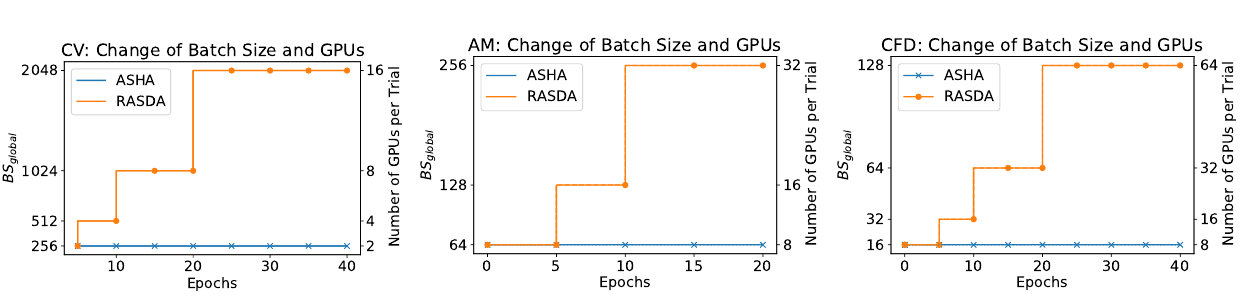
\includegraphics[width=\textwidth]{assets/trabalhos_relacionados/rasda_comparison.png}
\caption{Comparison of the global batch size and the number of GPUs per trial for ASHA and RASDA for the different application cases}
\caption*{Fonte: \citefigure{Aach2025}}
\label{fig:rasda_comparison}
\end{figure}

\subsection{Comparative Analysis of TensorFlow and PyTorch for Image Classification using CNN with Parallelism Strategies}

O segundo trabalho relacionado investiga o impacto de estratégias de paralelismo no treinamento de CNNs, comparando os principais frameworks de deep learning. Esta subseção analisa os resultados obtidos e as implicações para a escolha de ferramentas e estratégias de paralelização.

A escolha entre TensorFlow e PyTorch impacta a eficiência de classificação de imagens com redes neurais convolucionais. Este estudo investigou como estratégias de paralelismo de dados afetam o desempenho computacional e a acurácia dos modelos, comparando a MirroredStrategy do TensorFlow com a DataParallel do PyTorch nos datasets CIFAR-10 e CIFAR-100. A metodologia utilizou três camadas convolucionais seguidas por duas camadas densas. Cada framework foi testado em modo sequencial e com paralelismo de dados, coletando métricas de acurácia de teste, tempo de treinamento e curvas de aprendizado.

Os resultados do CIFAR-10 mostram que o paralelismo aumentou o tempo de treinamento devido à sobrecarga de comunicação: TensorFlow passou de 84,53s para 144,6s (Figura \ref{fig:tensorflow_results}), enquanto PyTorch foi de 210,42s para 253,2s (Figura \ref{fig:pytorch_results}). Apesar disso, o PyTorch manteve melhor acurácia com paralelismo (0,717 versus 0,680 do TensorFlow). As Figuras \ref{fig:tensorflow_results} e \ref{fig:pytorch_results} mostram como cada framework responde à introdução de paralelismo. No CIFAR-100 o paralelismo reduziu os tempos de treinamento: TensorFlow de 224,23s para 202,84s e PyTorch de 373,45s para 341,4s. O PyTorch escalou melhor em acurácia, aumentando de 0,43 para 0,45, enquanto o TensorFlow degradou de 0,46 para 0,42.

O estudo mostra que o TensorFlow é preferível para prototipagem rápida, enquanto o PyTorch se destaca em produção onde acurácia é prioritária. A eficácia do paralelismo depende da escala: em problemas menores, a sobrecarga anula os ganhos; em grande escala é necessário manter tempos de treinamento viáveis sem comprometer a qualidade preditiva.

\begin{figure}[H]
    \centering
    \captionsetup{justification=centering}
    \caption{Training and validation accuracy curves for TensorFlow using sequential and data parallelism strategies on CIFAR-10 dataset}
    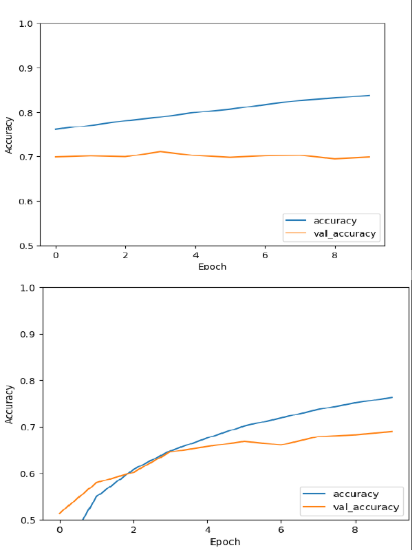
\includegraphics[width=0.4\textwidth]{assets/trabalhos_relacionados/comparative_analysis_of_tensorflow_and_pytorch_for_image_classification_using_cnn_with_parallelism_strategies_1.png}\\
    \captionsetup{justification=raggedright}
    \caption*{Fonte: \citefigure{Nandan10910577}}
    \label{fig:tensorflow_results}
\end{figure}

\begin{figure}[H]
    \centering
    \captionsetup{justification=centering}
    \caption{Training and validation accuracy curves for PyTorch using sequential and data parallelism strategies on CIFAR-10 dataset}
    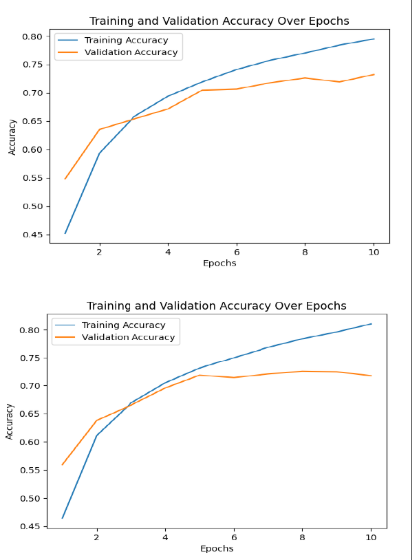
\includegraphics[width=0.4\textwidth]{assets/trabalhos_relacionados/comparative_analysis_of_tensorflow_and_pytorch_for_image_classification_using_cnn_with_parallelism_strategies_2.png}\\
    \captionsetup{justification=raggedright}
    \caption*{Fonte: \citefigure{Nandan10910577}}
    \label{fig:pytorch_results}
\end{figure}

\subsection{Avaliação de Fusão de Dados Espaciais com Espectrais para Classificação de Imagens Hiperespectrais}

O terceiro trabalho relacionado apresenta uma abordagem de fusão espectral-espacial para classificação de HSIs que serve como base metodológica para este estudo. Esta subseção analisa a arquitetura híbrida proposta e os resultados obtidos nos mesmos datasets utilizados neste trabalho.

No trabalho de \cite{Souza2023}, os autores abordam o desafio da classificação de Imagens Hiperespectrais (HSI), que enfrenta um trade-off entre complexidade computacional e acurácia. Métodos tradicionais focam em características espectrais, subutilizando a informação de contexto espacial que pode melhorar a distinção entre classes. Os objetivos são avaliar o impacto do pré-processamento espacial na classificação via aprendizado de máquina, integrar segmentação SEEDS com CNN 1D através de concatenação, comparar com modelos base e estado da arte, e quantificar o custo computacional dessa abordagem.

A metodologia propõe uma arquitetura híbrida que combina CNN 1D para classificação espectral com SEEDS para segmentação espacial. A Figura \ref{fig:metodologia_souza} ilustra o fluxo completo da metodologia proposta, desde a separação dos datasets até a extração das métricas de avaliação. O processamento ocorre em dois ramos paralelos: o ramo superior realiza PCA, definição de parâmetros, segmentação e concatenação das características espaciais; o ramo inferior executa PCA/vetorização, divisão dos dados de treino e classificação via CNN 1D. A CNN 1D possui 4 camadas Conv1D com 16, 32, 64 e 128 filtros, respectivamente, seguidas por 3 camadas Dense. A fusão ocorre via camada de concatenação que une as features extraídas pela CNN com o rótulo do superpixel correspondente.

\begin{figure}[H]
    \centering
    \captionsetup{justification=centering}
    \caption{Fluxograma da metodologia proposta mostrando o processamento paralelo dos dados espaciais e espectrais, seguido pela fusão via concatenação, classificação e validação iterativa do modelo}
    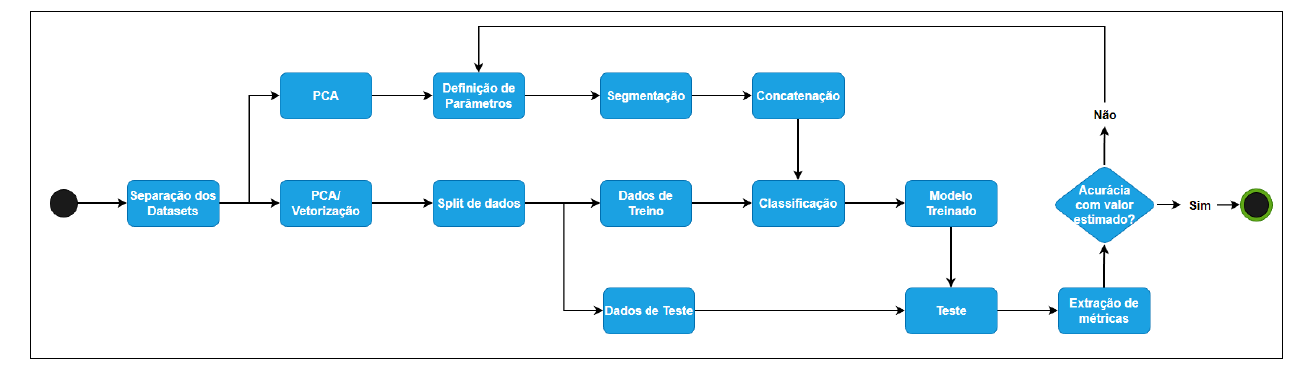
\includegraphics[width=\textwidth]{assets/trabalhos_relacionados/metodologia_souza.png}
    \captionsetup{justification=raggedright}
    \caption*{Fonte: \citefigure{Souza2023}}
    \label{fig:metodologia_souza}
\end{figure}

A validação experimental foi conduzida em três datasets: Indian Pines (21k pixels, 16 classes), Salinas Valley (111k pixels, 16 classes) e University of Pavia (207k pixels, 9 classes). As métricas avaliadas incluem Acurácia Global (OA), Acurácia Média (AA), coeficiente Kappa, tempo de inferência e uso de memória. O fluxograma da Figura \ref{fig:metodologia_souza} mostra ainda o processo iterativo de treinamento, teste e extração de métricas, com validação baseada em um valor estimado de acurácia.

\subsection{Análise Comparativa dos Trabalhos Relacionados}

A comparação sistemática entre os trabalhos relacionados permite identificar as lacunas na literatura e posicionar a contribuição deste estudo. Esta subseção apresenta uma análise comparativa destacando as principais diferenças em termos de arquitetura, processamento paralelo, segmentação, otimização de hiperparâmetros, métricas e tecnologias utilizadas.

O \autoref{tab:trabRel} demonstra as principais diferenças entre os trabalhos.

\begin{quadro}[H]
    \centering
    \caption{Comparação dos trabalhos relacionados}
    \resizebox{\textwidth}{!}{%
    \begin{tabular}{|p{0.20\textwidth}|p{0.19\textwidth}|p{0.19\textwidth}|p{0.19\textwidth}|p{0.19\textwidth}|}
        \hline
        \rowcolor[HTML]{EFEFEF}
        \textbf{Característica} & \textbf{\cite{Aach2025}} & \textbf{\cite{Nandan10910577}} & \textbf{\cite{Souza2023}} & \textbf{Este Trabalho} \\
        \hline
        \textbf{Arquitetura de IA} & 
        ResNet50/101/152 para ImageNet & 
        CNN customizada& 
        CNN 1D& 
        CNN 1D otimizada com fusão espacial-espectral \\
        \hline
        \textbf{Processamento Paralelo} & 
        Sim. RASDA& 
        Sim. Data Parallelism & 
        Não. Processamento sequencial & 
        Sim. Segmentação e CNN 1D paralelas via threads\\
        \hline
        \textbf{Segmentação} & 
        Não aplicado & 
        Não aplicado & 
        Sim. SEEDS ajustado manualmente & 
        Sim. SEEDS/LSC/Watershed com análise comparativa \\
        \hline
        \textbf{HPO} & 
        Sim. ASHA/RASDA.& 
        Não. Hiperparâmetros fixos& 
        Não. Ajuste manual empírico & 
        Sim. Grid Search/Bayesian Optimization para CNN e segmentação \\
        \hline
        \textbf{Métricas} & 
        Val MSE, Test MSE, Runtime, Relative Error & 
        Test Accuracy, Training Time, Val Accuracy & 
        OA, AA, Kappa, Tempo, Memória & 
        OA, AA, Kappa, Tempo, Memória, Speedup \\
        \hline
        \textbf{Datasets} & 
        ImageNet, CFD, RAISE-LPBF& 
        CIFAR-10, CIFAR-100& 
        Indian Pines, Salinas, Pavia& 
        Indian Pines, Salinas Valley, University of Pavia \\
        \hline
        \textbf{Tecnologias} & 
        Python, PyTorch, Horovod, DeepSpeed, Ray Tune, CUDA 11.5, NVIDIA DALI& 
        Python, TensorFlow, PyTorch, Keras, CUDA& 
        Python, TensorFlow, Keras, Scikit-Learn, OpenCV, Google Colab& 
        Python, TensorFlow, Keras, Scikit-Learn, OpenCV, Ray Tune, Google Colab/HPC\\
        \hline
    \end{tabular}%
    }
    \label{tab:trabRel}
\end{quadro}